%
%  untitled
%
%  Created by Johan Boissard [] on 2010-06-24.
%  Copyright (c) Johan Boissard. All rights reserved.
% hhh

\documentclass[a4paper] {scrartcl}
\usepackage[T1]{fontenc}
\usepackage[utf8]{inputenc}
\usepackage{graphicx}
\usepackage{engord}
%\usepackage[english]{babel}
\usepackage{fancyhdr}
\usepackage{amsmath}
\usepackage{comment}

\usepackage{listings}

%allows inclusion of url (hyperref is better than url) 
%ref: http://www.fauskes.net/nb/latextips/
\usepackage{hyperref}

%package for chemistry ie: \ce{(NH4)2SO4 -> NH4+ + 2SO4^2-} 
%ref:www.ctan.org/tex-archive/macros/latex/contrib/mhchem/mhchem.pdf
\usepackage[version=3]{mhchem}
%celsius + degrees
\usepackage{gensymb}
%to get last page
\usepackage{lastpage} % \pageref{LastPage}

%make use of the fullpage (no HUGE margins)
\usepackage{fullpage}
\usepackage{subfig}

%allows separating cell in table by diagonal line
\usepackage{slashbox}




%\renewcommand{\chaptername}{Laboratory}
%\setcounter{chapter}{5}

\usepackage{color}
\usepackage[usenames,dvipsnames, table]{xcolor}
% Include this somewhere in your document



\usepackage[absolute]{textpos}

%column  of multi row in tables
\usepackage{multirow}

%to have vertical text in table
\usepackage{rotating}


%%tikz
\usepackage{tikz}
\usetikzlibrary{arrows,calc}
\usepackage{relsize}
\newcommand\LM{\ensuremath{\mathit{LM}}}
\newcommand\IS{\ensuremath{\mathit{IS}}}

%%%%%%% a virer ici!!!!
\begin{comment}
%Fonts and Tweaks for XeLaTeX
\usepackage{fontspec,xltxtra,xunicode}
%\defaultfontfeatures{Mapping=tex-text}
%\setromanfont[Mapping=tex-text]{Hoefler Text}
\setsansfont[Scale=MatchLowercase,Mapping=tex-text]{Gill Sans}

\definecolor{shade}{HTML}{D4D7FE}	%light blue shade
\definecolor{text1}{HTML}{272727}		%text is almost black
\definecolor{headings}{HTML}{173849} 	%dark blue %%%dark red 70111
\definecolor{title}{HTML}{173849} 	%dark blue %%%dark red 70111

\usepackage{titlesec}				%custom \section
\end{comment}







\author{Johan Boissard - 06-304-679}
\date{\today}
\title{MacroEconomics - HW1}
\begin {document}

\maketitle
%\tableofcontents


%%1
\section{ }
\subsection{ }
LM-curve is (at equilibrium $L=M=\overline M$)
\begin{equation}
	i = \frac{k}{h}Y-\frac{1}{h}\overline M
\end{equation}
IS-curve is ($Y = C+I+G+NX$ and solving for $i$)
\begin{equation}
	i = -\frac{1-c+m_1}{b}Y+ \frac{\overline I + G + x_1Y^{\text{world}}}{b}+\frac{x_2+m_2}{b}R
\end{equation}
at the equilibrium the interest rate is the same $i_{IS} = i_{LM}$, thus solving for $Y$ gives
\begin{equation}
	Y = %\underbrace{
	\frac{1}{kb+h(1-c+m_1)}
	%}_{MPC}
			\left(b\overline M+h
				\left(\overline I+G+x_1Y^{\text{world}}+(x_2+m_2)R\right)
			\right)
\end{equation}

\subsection{ }
\subsubsection{ }
An increase in money supply will raise income (more money available) and decrease $i$ (people no longer have a high interest rate), please see fig \ref{fig:ISLM1}
\begin{figure}[htbp]
	\centering
		
	

\begin{tikzpicture}[
        scale=2,
        IS/.style={blue, thick},
        LM/.style={red, thick},
        axis/.style={very thick, ->, >=stealth', line join=miter},
        important line/.style={thick}, dashed line/.style={dashed, thin},
        every node/.style={color=black},
        dot/.style={circle,fill=black,minimum size=4pt,inner sep=0pt,
            outer sep=-1pt},
    ]
    % axis
    \draw[axis,<->] (2.5,0) node(xline)[right] {$Y$} -|
                    (0,2.5) node(yline)[above] {$i$};
	
	%LM
	\draw[important line, red, xshift=.1cm]
	            (.1,.1) coordinate (es) -- (1.7,2) coordinate (ee)
	            node [above right] {$LM$};
	
	%LM after shift
	\draw[important line, red, xshift=.1cm]		         
	   (.6,.1) coordinate (es) -- (2.3,2) coordinate (ee)
	   node [above right] {$LM'$};
	
	%IS
	\draw[important line, blue, xshift=.1cm]
	            (.1,2) coordinate (es) -- (1.7,.2) coordinate (ee)
	            node [above right] {$IS$};
	
	\node[dot,label=above:$A$] at (1.02,1.1) (int1) {};
	\node[dot,label=above:$B$] at (1.32,.8) (int1) {};
	
	\draw[->, very thick, black, >=stealth']
       (1.2,1.3) -- (1.5,1)
        node[sloped, above, midway] {$\mathsmaller{\Delta M > 0}$};
\end{tikzpicture}
\caption{shift caused by an increase in Money supply}
\label{fig:ISLM1}
\end{figure}

\subsubsection{ }
An increase in $R$ see fig \ref{fig:ISLM2} gives rise to a better interest rate and a higher income. Indeed have more buying power so they can afford more ($Y$ goes up) and thus consume more $i$ goes up.
\begin{figure}[htbp]
	\centering
		
	

\begin{tikzpicture}[
        scale=2,
        IS/.style={blue, thick},
        LM/.style={red, thick},
        axis/.style={very thick, ->, >=stealth', line join=miter},
        important line/.style={thick}, dashed line/.style={dashed, thin},
        every node/.style={color=black},
        dot/.style={circle,fill=black,minimum size=4pt,inner sep=0pt,
            outer sep=-1pt},
    ]
    % axis
    \draw[axis,<->] (2.5,0) node(xline)[right] {$Y$} -|
                    (0,2.5) node(yline)[above] {$i$};
	
	%LM
	\draw[important line, red, xshift=.1cm]
	            (.1,.1) coordinate (es) -- (1.7,2) coordinate (ee)
	            node [above right] {$LM$};
	

	
	%IS
	\draw[important line, blue, xshift=.1cm]
	            (.1,2) coordinate (es) -- (1.7,.2) coordinate (ee)
	            node [above right] {$IS$};
	
	%IS after shift
	\draw[important line, blue, xshift=.1cm]
	            (.5,2.4) coordinate (es) -- (2.1,.6) coordinate (ee)
	           node [above right] {$IS'$};
	
	\node[dot,label=above:$A$] at (1.02,1.1) (int1) {};
	\node[dot,label=above:$B$] at (1.36,1.53) (int1) {};
	
	\draw[->, very thick, black, >=stealth']
       (.9,1.2) -- (1.3,1.6)
        node[sloped, above, midway] {$\mathsmaller{\Delta R > 0}$};
\end{tikzpicture}
\caption{shift caused by an increase in $R$}
\label{fig:ISLM2}
\end{figure}

\subsection{ }
The curve will become steeper. Which means that effects after a shift in the $LM$ curve will be stronger on the interest rate and less important on the income $Y$. See fig \ref{fig:ISLM3}
\begin{figure}[htbp]
	\centering
		
	

\begin{tikzpicture}[
        scale=2,
        IS/.style={blue, thick},
        LM/.style={red, thick},
        axis/.style={very thick, ->, >=stealth', line join=miter},
        important line/.style={thick}, dashed line/.style={dashed, thin},
        every node/.style={color=black},
        dot/.style={circle,fill=black,minimum size=4pt,inner sep=0pt,
            outer sep=-1pt},
    ]
    % axis
    \draw[axis,<->] (2.5,0) node(xline)[right] {$Y$} -|
                    (0,2.5) node(yline)[above] {$i$};
	
	%LM
	\draw[important line, red, xshift=.1cm]
	            (.1,.1) coordinate (es) -- (1.7,2) coordinate (ee)
	            node [above right] {$LM$};
	

	
	%IS
	\draw[important line, blue, xshift=.1cm]
	            (.1,2) coordinate (es) -- (1.7,.2) coordinate (ee)
	            node [above right] {$IS$};
	
	%IS after shift
	\draw[important line, blue, xshift=.1cm]
	            (.5,2.4) coordinate (es) -- (1.2,.2) coordinate (ee)
	           node [above right] {$IS'$};
	
	\node[dot,label=above:$A$] at (1.02,1.1) (int1) {};
%	\node[dot,label=above:$B$] at (1.36,1.53) (int1) {};
	
	%\draw[->, very thick, black, >=stealth']
     %  (.9,1.2) -- (1.3,1.6)
      %  node[sloped, above, midway] {$\mathsmaller{\Delta R > 0}$};
\end{tikzpicture}
\caption{Illustration of a decrease in $c$}
\label{fig:ISLM3}
\end{figure}


%%1.4
\subsection{}


In this model, $Y, i, R$ are endogenous variables. If we know set $i = \overline i$, $i$ becomes an endogenous variable and we only have two endogenous variables left ($Y$ and $R$) and two equations. This means that there are no degrees of freedom left and the equilibrium is determined.

Mathematically, it is
\begin{equation}
	Y^* = \frac{h}{k}\overline i+\overline M 
\end{equation}
for the equilibrium income and
\begin{equation}
	R^* = \frac{1}{x_2+m_2}\left[b\overline i+(1-c+m_1)Y^*-(\overline I+g+x_1Y^{\text{world}})\right]
\end{equation}
for the exchange rate.

This can be represented on a graph like on fig \ref{fig:ISLMwE} (note that the $LM$ curve is not dependent on $R$ thus it is simply a vertical line).

\begin{figure}[htbp]
	\centering
		
	

\begin{tikzpicture}[
        scale=2,
        IS/.style={blue, thick},
        LM/.style={red, thick},
        axis/.style={very thick, ->, >=stealth', line join=miter},
        important line/.style={thick}, dashed line/.style={dashed, thin},
        every node/.style={color=black},
        dot/.style={circle,fill=black,minimum size=4pt,inner sep=0pt,
            outer sep=-1pt},
    ]
    % axis
    \draw[axis,<->] (2.5,0) node(xline)[right] {$Y$} -|
                    (0,2.5) node(yline)[above] {$R$};
	
	%LM
	\draw[important line, blue, xshift=.1cm]
	            (.1,.1) coordinate (es) -- (1.7,2) coordinate (ee)
	            node [above right] {$IS$};
	

	
	%IS
	\draw[important line, red, xshift=.1cm]
	            (1,.1) coordinate (es) -- (1,2.2) coordinate (ee)
	            node [above right] {$LM$};
	

	\node[dot,label=above:$A$] at (1.12,1.17) (int1) {};
%	\node[dot,label=above:$B$] at (1.36,1.53) (int1) {};
	
	%\draw[->, very thick, black, >=stealth']
     %  (.9,1.2) -- (1.3,1.6)
      %  node[sloped, above, midway] {$\mathsmaller{\Delta R > 0}$};
\end{tikzpicture}
\caption{Equilibrium variables for $R$ and $Y$}
\label{fig:ISLMwE}
\end{figure}



%%1.5
\subsection{ }
%In the casecase the interest rate rule is $i = \overline i -b\overline Y+bY$, the $LM$-curve becomes
%\begin{equation}
%	i = \frac{k}{h}Y-\frac{1}{h}M
%\end{equation}
%where $M\neq\overline M$ and has become an exogenous variable.


\begin{figure}[htbp]
	\centering
		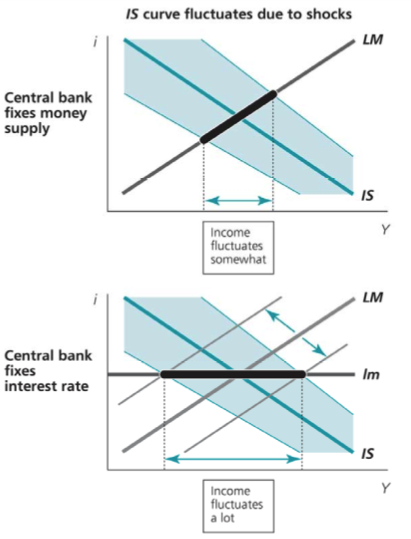
\includegraphics[height=4.5in]{fluc.png}
	\caption{Effects of policy instruments on the income (from Gaertner)}
	\label{fig:fluc}
\end{figure}

In the case where the central bank fixes the money supply ($M=\overline M$), the $IS$-curve fluctuates around the $LM$-curve but the difference in the $IS$-curve is damped by the slope of the $LM$-curve which can't move (no endogenous variable that is not $i$ or $Y$). This results in an income ($Y$) that "fluctuates somewhat", see fig \ref{fig:fluc} top for graphical representation (taken from Gärtner, chapter 3).

On the other hand, when the interest rate is fixed, the $LM$-curve becomes
\begin{equation}
	i = \frac{k}{h}Y-\frac{1}{h}M
\end{equation}
where $M\neq\overline M$ and has become an endogenous variable. In this case the $LM$-curve, since it has an endogenous variable, can respond to the shift of the $IS$-curve. This results in an "income that fluctuates a lot", see fig \ref{fig:fluc} bottom.

\subsubsection{Formally}


For the fixed money supply, we have (rewriting in a simpler manner)
\begin{eqnarray}
	i&=& 
	%\frac{k}{h}Y-\frac{1}{h}\overline M =
	aY  -b\label{eq:LM}\\
	i&=& -cY+d_0\label{eq:IS}
\end{eqnarray}
where $a,b,c,d>0$, \ref{eq:LM} is the $LM$-curve
and \ref{eq:IS} is the $IS$-curve. 

At equilibrium, we have
\begin{equation}
	Y^* = \frac{d_0+b}{a+c}
\end{equation}

If $IS$ moves, the change is 
\begin{equation}
	\label{eq:chg}
	\Delta i = d_1 - d_0 = \Delta d
\end{equation}

Thus the new equilibrium becomes
\begin{equation}
	Y^* = \frac{d_1+b}{a+c}
\end{equation}
and the change is
\begin{equation}
	\label{eq:chg1}
	\Delta Y^* = \frac{\Delta d}{a+c}
\end{equation}

Now, if the interest rate is fixed, we have 
\begin{eqnarray}
	\overline i&=& 
	%\frac{k}{h}Y-\frac{1}{h}\overline M =
	aY  -b_0\label{eq:LM}\\
	\overline i&=& -cY+d_0\label{eq:IS}
\end{eqnarray}
where $a,b,c,d>0$, \ref{eq:LM} is the $LM$-curve
,\ref{eq:IS} is the $IS$-curve and $b=\frac{1}{h}M$.

Now, if the $IS$-curve moves, the change is the same as before (see eq \ref{eq:chg}) but the $LM$ curve will compensate by the same amount through a change in the money supply described here by $b$; this is so because $\overline i$ can't change. Thus we have
\begin{equation}
	\Delta i = -(d_1-d_0)=-\Delta d
\end{equation}



Taking in account the latter, the variation in income rewrites
\begin{equation}
	\label{eq:chg2}
	\Delta Y^* = \frac{2\Delta d}{a+c}
\end{equation}

By looking at eq \ref{eq:chg1} and eq \ref{eq:chg2}, one immediately notices that the change is always bigger when the central bank fixes interest rate, and this is also in accordance with figure \ref{fig:fluc}.


%%2
\section{ }
\subsection{ }
The equilibrium is not reached: the $FE$, $LM$ and $IS$-curves do not cross at one single point. What happens economically is that the interest rate ($i$) is too high compared to the $i^{\text{world}}$, consequently the rest of the world has an incentive to invest in the domestic country which will eventually bring down the equilibrium towards $i^{\text{world}}$, either by decreasing $R$ ($IS$-curve) or by increasing $\overline M$ (depends on policy).

\subsection{ }
For this sub-exercise we assume the $FE$-curve to be $i=i^{\text{world}}$
\subsubsection{flexible exchange rate}
Under flexible exchange rate, the endogenous variables of the model are $R, i, Y$ and policy makers can only influence $R$ directly. Since only the $IS$-curve is dependent on this variable, $R$ needs to decrease so that the whole $IS$-curve goes down and eventually reaches the equilibrium. See fig \ref{fig:ex21}
\begin{figure}[htbp]
	\centering
		\begin{tikzpicture}[
		        scale=2,
		        IS/.style={blue, thick},
		        LM/.style={red, thick},
		        axis/.style={very thick, ->, >=stealth', line join=miter},
		        important line/.style={thick}, dashed line/.style={dashed, thin},
		        every node/.style={color=black},
		        dot/.style={circle,fill=black,minimum size=4pt,inner sep=0pt,
		            outer sep=-1pt},
		    ]
		    % axis
		    \draw[axis,<->] (2.5,0) node(xline)[right] {$Y$} -|
		                    (0,2.5) node(yline)[above] {$i$};

			%LM
			\draw[important line, red, xshift=.1cm]
			            (.1,.1) coordinate (es) -- (1.7,2) coordinate (ee)
			            node [above right] {$LM$};



			%IS
			\draw[important line, blue, xshift=.1cm]
			            (.1,2) coordinate (es) -- (1.7,.2) coordinate (ee)
			            node [above right] {$IS'$};

			%IS after shift
			\draw[important line, blue, xshift=.1cm]
			            (.5,2.4) coordinate (es) -- (2.1,.6) coordinate (ee)
			           node [above right] {$IS$};
			
			%FE
			\draw[important line, green, xshift=.1cm]
			            (.1,1.1) coordinate (es) -- (2.1,1.1) coordinate (ee)
			           node [above right] {$FE$};

			\node[dot,label=above:$B$] at (1.02,1.1) (int1) {};
			\node[dot,label=above:$A$] at (1.36,1.53) (int1) {};

			\draw[->, very thick, black, >=stealth']
		        (1.3,1.6) -- (.9,1.2)
		        node[sloped, above, midway] {$\mathsmaller{\Delta R < 0}$};
		\end{tikzpicture}
\caption{$IS$ curve decrease and reaches equilibrium}
\label{fig:ex21}
\end{figure}


\subsubsection{fixed exchange rate}
Under fixed exchange rate, the endogenous variables are $i, Y, M$. Once again $i, Y$ can't be controlled directly, thus the $LM$-curve (since it is the only one dependent on $M$) goes down ($\Delta M>0$), see fig \ref{fig:ex22}.

\begin{figure}[htbp]
	\centering
		
	

\begin{tikzpicture}[
        scale=2,
        IS/.style={blue, thick},
        LM/.style={red, thick},
        axis/.style={very thick, ->, >=stealth', line join=miter},
        important line/.style={thick}, dashed line/.style={dashed, thin},
        every node/.style={color=black},
        dot/.style={circle,fill=black,minimum size=4pt,inner sep=0pt,
            outer sep=-1pt},
    ]
    % axis
    \draw[axis,<->] (2.5,0) node(xline)[right] {$Y$} -|
                    (0,2.5) node(yline)[above] {$i$};
	
	%LM
	\draw[important line, red, xshift=.1cm]
	            (.1,.1) coordinate (es) -- (1.7,2) coordinate (ee)
	            node [above right] {$LM$};
	
	%LM after shift
	\draw[important line, red, xshift=.1cm]		         
	   (.6,.1) coordinate (es) -- (2.3,2) coordinate (ee)
	   node [above right] {$LM'$};
	
	%IS
	\draw[important line, blue, xshift=.1cm]
	            (.1,2) coordinate (es) -- (1.7,.2) coordinate (ee)
	            node [above right] {$IS$};
	
				%FE
				\draw[important line, green, xshift=.1cm]
				            (.1,.8) coordinate (es) -- (2.1,.8) coordinate (ee)
				           node [above right] {$FE$};
	
	\node[dot,label=above:$A$] at (1.02,1.1) (int1) {};
	\node[dot,label=above:$B$] at (1.32,.8) (int1) {};
	
	
	
	\draw[->, very thick, black, >=stealth']
       (1.2,1.3) -- (1.5,1)
        node[sloped, above, midway] {$\mathsmaller{\Delta M > 0}$};
\end{tikzpicture}
\caption{Increasing $M$ shifts the $FE$-curve down eventually reaching equilbirium ($B$)}
\label{fig:ex22}
\end{figure}

%%3
\section{ }
\label{sec:prob3}
\paragraph{Large Economy} % (fold)
\label{par:large_economy}
A global economy model means that $NX=0$ and that the interest rate $i$ is the world's interest rate ($i= i^{\text{world}}$). 
Thus the $FE$-curve is irrelevant in this context and we reduce our analysis only to the $IS$ and $LM$ curve that writes, in this case, as follows
\begin{eqnarray}
	i_{LM} &=& aY-b\\
	i_{IS} &=& -cY+d+eG
\end{eqnarray}
where the constants ($R$ assumed constant) and unused variables for this problem are hidden in $a,b,c,d,e>0$.
% paragraph large_economy (end)

\paragraph{Small economy} % (fold)
\label{par:small_economy}
Since the small economy relies on the large economy (the world's interest rate is determined by the large economy), we need to take in account the $FE$-curve ($i=i^{\text{world}}$ because of perfectly mobile capital).

The $IS$ and $LM$ curves writes as for the global economy with exception that they have to equal $i^{world}\neq i$
% paragraph small_economy (end)

\paragraph{Solution} % (fold)
\label{par:solution}
If there is an expansionary tax policy, this means that $G$ is increased, and thus the $IS$ curve of the global economy goes up leading to a higher income and a higher interest rate. This new interest rate is also the new $i^{\text{world}}$ which means that the $FE$ curve of the small economy ($i=i^{\text{world}}$) has to shift up to adapt to this new interest rate. This in turns obliges either the $IS$ or the $LM$ curve to shift respectively to the right or to the left. However, $R$ is kept constant so the only endogenous variable left is the money supply $M$ that has to decrease to permit the equilibrium to be reached. Since only the $LM$ curve shift, and shift to the right, the small economy will suffer from a lower income with a higher interest rate. The situation is depicted in figures \ref{fig:ex31} and \ref{fig:ex32}.
% paragraph solution (end)



\begin{figure}
  \centering
  	\subfloat[Global/large economy]{\label{fig:ex31}
	
	%\includegraphics[width=0.3\textwidth]{gull}
	\begin{tikzpicture}[
	        scale=2,
	        IS/.style={blue, thick},
	        LM/.style={red, thick},
	        axis/.style={very thick, ->, >=stealth', line join=miter},
	        important line/.style={thick}, dashed line/.style={dashed, thin},
	        every node/.style={color=black},
	        dot/.style={circle,fill=black,minimum size=4pt,inner sep=0pt,
	            outer sep=-1pt},
	    ]
	    % axis
	    \draw[axis,<->] (2.5,0) node(xline)[right] {$Y$} -|
	                    (0,2.5) node(yline)[above] {$i$};

		%LM
		\draw[important line, red, xshift=.1cm]
		            (.1,.1) coordinate (es) -- (1.7,2) coordinate (ee)
		            node [above right] {$LM$};



		%IS
		\draw[important line, blue, xshift=.1cm]
		            (.1,2) coordinate (es) -- (1.7,.2) coordinate (ee)
		            node [above right] {$IS$};

		%IS after shift
		\draw[important line, blue, xshift=.1cm]
		            (.5,2.4) coordinate (es) -- (2.1,.6) coordinate (ee)
		           node [above right] {$IS'$};

		\node[dot,label=above:$A$] at (1.02,1.1) (int1) {};
		\node[dot,label=above:$B$] at (1.36,1.53) (int1) {};

		\draw[->, very thick, black, >=stealth']
	       (.9,1.2) -- (1.3,1.6)
	        node[sloped, above, midway] {$\mathsmaller{\Delta G > 0}$};
	\end{tikzpicture}
	}                
	
	\subfloat[Small economy]{\label{fig:ex32}
	%\includegraphics[width=0.3\textwidth]{tiger}
	\begin{tikzpicture}[
	        scale=2,
	        IS/.style={blue, thick},
	        LM/.style={red, thick},
	        axis/.style={very thick, ->, >=stealth', line join=miter},
	        important line/.style={thick}, dashed line/.style={dashed, thin},
	        every node/.style={color=black},
	        dot/.style={circle,fill=black,minimum size=4pt,inner sep=0pt,
	            outer sep=-1pt},
	    ]
	    % axis
	    \draw[axis,<->] (2.5,0) node(xline)[right] {$Y$} -|
	                    (0,2.5) node(yline)[above] {$i$};

		%LM
		\draw[important line, red, xshift=.1cm]
		            (.1,.1) coordinate (es) -- (1.7,2) coordinate (ee)
		            node [above right] {$LM'$};

		%LM after shift
		\draw[important line, red, xshift=.1cm]		         
		   (.6,.1) coordinate (es) -- (2.3,2) coordinate (ee)
		   node [above right] {$LM$};

		%IS
		\draw[important line, blue, xshift=.1cm]
		            (.1,2) coordinate (es) -- (1.7,.2) coordinate (ee)
		            node [above right] {$IS$};

					%FE
					\draw[important line, green, xshift=.1cm]
					            (.1,.8) coordinate (es) -- (2.1,.8) coordinate (ee)
					           node [above right] {$FE$};
					
							%FE
							\draw[important line, green, xshift=.1cm]
							            (.1,1.1) coordinate (es) -- (2.1,1.1) coordinate (ee)
							           node [above right] {$FE'$};

		\node[dot,label=above:$B$] at (1.02,1.1) (int1) {};
		\node[dot,label=above:$A$] at (1.32,.8) (int1) {};



		\draw[->, very thick, black, >=stealth']
	        (1.5,1) -- (1.2,1.3)
	        node[sloped, above, midway] {$\mathsmaller{\Delta M < 0}$};
	\end{tikzpicture}
	}
  \caption{Illustration of the problem \ref{sec:prob3}}
  \label{fig:animals}
\end{figure}


%%4
\section{ }
\subsection{ }
We have
\begin{eqnarray}
	\Delta L &=& -sL+fU+(1-e_u)eN-(1-q_u)qN\\
	\Delta U &=& sL-fU+e_ueN-q_uqN
\end{eqnarray}
the equilibtrium condition reads $\Delta U=0$ and thus
\begin{equation}
	fU^* = sL+e_ueN-(1-q_u)qN
\end{equation}
dividing by $N$ gives
\begin{equation}
	fu^* = s\frac{L}{N}+e_ue-q_uq
\end{equation}
substituting $\frac{E}{N}$ by $(1-u^*)$ leads to
\begin{equation}
	fu^*= s(1-u^*) +e_ue-q_uq
\end{equation}
and thus
\begin{equation}
	u^* = \frac{1}{s+f}\left(s+e_ue-q_uq\right)
\end{equation}

\subsection{ }
\begin{eqnarray}
	\frac{\partial u^*}{\partial f} &=& -\frac{1}{(s+f)^2}\left(s+e_ue-q_uq\right)\\
	&=&  -\frac{1}{s+f}u^*
\end{eqnarray}
Thus as long as $u^*>0$, $u^*$ will decrease when $f$ increase. Intuitively, this seems reasonable: if the finding rate increase, logically the unemployment should decrease. 

\subsection{ }
\begin{eqnarray}
	\frac{\partial^2u^*}{\partial f\partial s}
	&=&
	%\frac{s-f}{(s+f)^3}+2\frac{1}{(s+f)^3}(e_ue+(1-qu)q)
	\frac{s-f+2(e_ue-q_uq)}{(s+f)^3}
\end{eqnarray}
Since $s>f-2(e_ue-q_uq)$ the expression is strictly positive (we assume $s,f>0$). This means that an increase in $s$ will make $\frac{\partial u^*}{\partial f}$ bigger and thus an increase in the separation rate gives a higher unemployment rate for the same $f$ in other words $s$ compensates with $f$.

\section{ }
%Foreign inflation  NX rises (foreign goods more expensive, domestic ones cheaper) AD shifts
To keep the exchange rate constant ($R=E\frac{P^{\text{world}}}{P}$) the domestic price level ($P$) must adjust to the world price level ($P^{\text{world}}$). In this case, $P$ increase and thus the growth rate increase going from $\mu_{LO}$ to $\mu_{HI}$ this is reflected by the upward shift of $EAD$ ($EAD_{old}$ to $EAD_{new}$ on fig \ref{fig:images_adapExp} and $EAD_{LO}$ to $EAD_{hi}$ on fig \ref{fig:images_ratExp}).

\subsection{Adaptive expectation}

\begin{figure}[htbp]
	\centering
		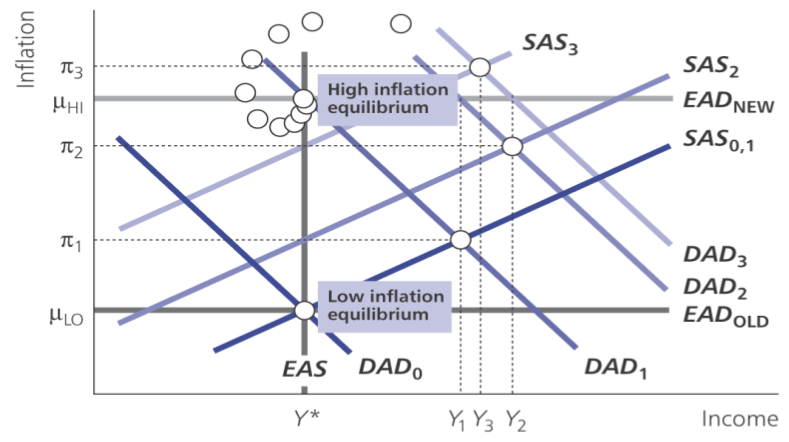
\includegraphics[height=2.5in]{images/adapExp.png}
	\caption{Effect of an increase of $\mu$ with people having an adaptive expectation (from Gaertner)}
	\label{fig:images_adapExp}
\end{figure}



With adaptive expectations people don't know the model that is behind and behave based on what happened in the past.

At first the $DAD$ will move up to cross the new the $EAD$ curve. This give rise to a new income $Y_1$ and $\pi_1$. In the next cycle, the labor force noticed that the inflation is higher and thus negotiate higher wages which utlimately lead to a new $DAD$ curve that cross the $EAS$ curve at $\pi_1$ but at the same time $DAD$ moves also to the point where $EAD=Y_1$. This keeps going on like this until it reaches the new equilibrium (on the long run) $(Y^*,\mu_{HI})$. The effect is graphically depicted on fig \ref{fig:images_adapExp}.


\subsection{Rational expectation}

\begin{figure}[htbp]
	\centering
		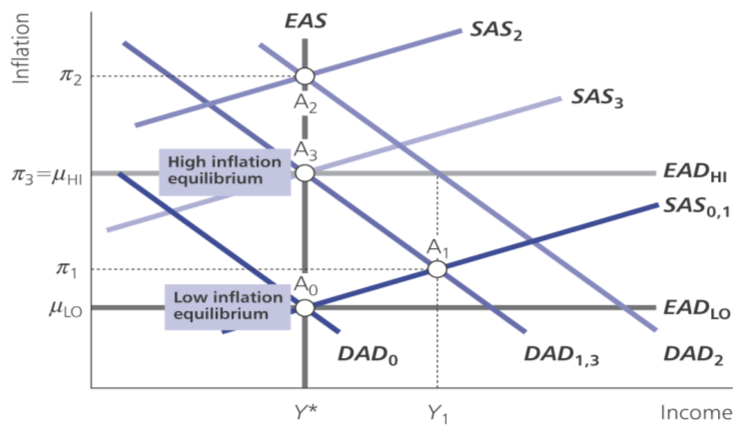
\includegraphics[height=2.5in]{images/ratExp.png}
	\caption{Effect of an increase of $\mu$ with people having an rational expectation (from Gaertner)}
	\label{fig:images_ratExp}
\end{figure}

Here, people understand the model and will behave accordingly.

In the first period, $DAD$ moves up from $\mu_{LO}$ to $\mu_{HI}$, the $SAS$ does not move as change in the money supply can not be foreseen. Thus, the output is $Y_1>Y^*$ and the inflation rate is also larger $\pi_1>\mu_{LO}$ but still not as high as the new one ($\pi_1<\mu_{HI}$).

In the second phase, as people know the model they can anticipate. $DAD_2$ has to cross the $EAD$ at $Y_1$. If people want the output to come back to $Y^*$, $DAD_2$ and $SAS_2$ have to cross at the $EAS$. This leads to an output $Y_2=Y^*$ but an inflation rate ($\pi_2$) that is this time higher than $\mu_{HI}$.

In the last period $SAS_3$ adjusts via $Y^*$ and the $EAD$ curve. $SAS_3$ is corrected by the same amount. Hence the equilibrium (where $EAD$ and $EAS$ cross, $(Y^*,\mu_{HI})$) is reached.

The effect is graphically depicted on fig \ref{fig:images_ratExp}.

Note that for the two cases, the equilibrium is the same on the long-run. But the adaptive expectation mechanism takes longer to reach the equilibrium and causes more fluctuations whereas in the rational expectation mechanism it takes only 3 steps to reach the equilibrium.

\end{document}
